% !TEX root = ../main.tex
\section{Introduction}

In late 2024, the United States was in the midst of a presidential election when the decentralized prediction market, Polymarket~\cite{poly}, broke through mainstream news coverage~\cite{YBG24,Cha24}. Stories focused, in particular, on the fact that it offered odds more favourable to eventual winner Donald Trump than those reflected in conventional polls and forecasts. Polymarket's odds are not set by experts or pundits, instead it is a specific type of betting market where odds are extrapolated from the prices of trades made in an open market (or somewhat open, as Polymarket was banned at the time in many countries including the US). 

As with traditional betting, whether online or through a bookie, prediction markets allow speculators to profit from correct forecasts~\cite{AFGH+08,WoZi06}. However the structure of a prediction market is different than traditional betting. One key difference is that prediction markets ease the process of moving in and out of bets before the event resolves, encouraging traders to place bets if they think the odds are over- or under-stated, and withdrawing profits if the odds realign.

It would be easy to think that Polymarket's design is the most obvious, straight-forward way to deploy a decentralized prediction market (\depm) on a blockchain. However the central thesis of this systemization of knowledge (SoK) paper is that Polymarket found success in bucking the trend. \depms were first given a few paragraphs in the Ethereum vision paper~\cite{But13}, released in late 2013 for the blockchain that would be deployed in 2015. Then two 2014 papers presented flushed out systems: a whitepaper called Truthcoin~\cite{Sz14} and an academic paper at WEIS 2014~\cite{BCFKMN14} (informally known as the `Princeton \depm' because of author affiliation). Developed independently,\footnote{The Princeton paper describes Truthcoin as being released while the paper was under review~\cite{BCFKMN14}, and the Truthcoin FAQ~\cite{Sz14b} mentions hearing about the Princeton paper but not having found the paper itself.} the two papers' designs are vastly different, representing two different goalposts for how a \depm might look. 

Early systems, like Augur~\cite{AKPWZ15} and Gnosis~\cite{Gn17} closely resembled Truthcoin~\cite{Sz14}, while modern systems like Polymarket~\cite{poly} either resemble the Princeton \depm~\cite{BCFKMN14} or use new solutions that resemble a hybrid of the two designs. Consider some examples:

\begin{enumerate}
\item From \S\ref{wf:price}, in Truthcoin, the market creator is active in setting initial prices (\ie odds) for each option and risks its own money (bounded)~\cite{Sz14}. In the Princeton system, the market creator is passive, not setting prices or risking any money~\cite{BCFKMN14}. Polymarket uses the latter~\cite{poly}. 

\item From \S\ref{wf:trade}, in Truthcoin, outcome shares are created with predecessor to an automated market maker~\cite{Sz14}. In the Princeton \depm, outcome shares are traded with an orderbook~\cite{BCFKMN14}. In Polymarket, outcome shares can be traded with either an AMM or an orderbook~\cite{poly}. 

\item From \S\ref{wf:close}, in Truthcoin, the blockchain decides event outcomes (\eg who won the election) through a reputation-based on-chain vote with slashing~\cite{Sz14}. In the Princeton paper, they are resolved through trusted arbiters acting as oracles~\cite{BCFKMN14}. The Ethereum whitepaper suggests both~\cite{But13}. In Polymarket, the third party oracle, UMA, operates under the hood through on-chain voting with slashing, but only when outcomes are disputed~\cite{poly,uma}.
\end{enumerate}

Noticing these points of differences inspired us to ask what are all the design decisions involved in creating a \depm?  We reviewed over a hundred designs, distilled into the 35+ notable \depms listed in Appendix~\ref{app:list}. We break the \depm design space into a `modular workflow' (the method used in an SoK at AFT 2021 on oracles~\cite{ClEsGS21}) with seven stages: underlying infrastructure, market topic, share structure and pricing, trading, market resolution, settlement, and archiving. For each stage, we enumerate the possible designs and discuss competing trade-offs. 

% ChatGPT generated timeline so cross-validate everything before believing any of it:
%	•	1988 — Iowa Electronic Markets (IEM) launch as an academic, real-money prediction market at the University of Iowa.   
%	•	1990–2003 — Robin Hanson foundation work: “Idea Futures” concept (1990s) and the logarithmic market scoring rule (LMSR) (2002/03), which becomes the standard automated market maker design for PMs.  
%	•	2003 — Policy Analysis Market (PAM) (DARPA) announced then quickly canceled amid controversy; keeps prediction markets in the policy spotlight.   
%	•	2012–2013 — Intrade exits U.S. and then shuts down following a CFTC lawsuit (Nov 26, 2012) and subsequent turmoil (site shutdown Mar 10, 2013).    
%	•	2013–2014 — Ethereum vision includes prediction markets as a core smart-contract use case.  
%	•	2014 — Princeton/WEIS paper “On Decentralizing Prediction Markets and Order Books” sketches a Bitcoin-based design; a seminal academic reference for on-chain PMs.  
%	•	2014–2015 — Truthcoin / Hivemind (Paul Sztorc) proposes a Bitcoin sidechain oracle + PM protocol (whitepaper v1.5 dated Dec 2015; early drafts 2014).   
%	•	2015 — Augur token sale (~$5M) to build a decentralized oracle + PM on Ethereum.  
%	•	2016–2017 — Gnosis forms & conducts ICO (2017) to pursue PMs and related tooling on Ethereum.  
%	•	2018 — Augur v1 goes live on Ethereum (first major decentralized PM on mainnet).  
%	•	2018 — Kleros launches (Ethereum-based decentralized court), later widely used with Reality.eth as an oracle stack for PM-style applications.   
%	•	2020 — Augur v2 launches (DAI-denominated, faster resolution; “Invalid” tradable), marking a big UX/market-mechanics upgrade.  
%	•	2020 — Omen (by Gnosis) launches a PM front-end using the Conditional Tokens Framework on xDai/Gnosis Chain.  
%	•	2020 — Polymarket launches and grows rapidly; runs on Polygon PoS and (today) resolves via UMA’s Optimistic Oracle.   
%	•	2021 — Augur Turbo launches on Polygon with sports & rapid markets.  
%	•	2021–2024 — Zeitgeist launches as a PM parachain on Kusama and migrates to Polkadot in 2024.  
%	•	2022 — CFTC settles with Polymarket (geoblocks U.S. users; continues ex-U.S.).  
%	•	2020 onward — GnosisDAO experiments with futarchy, i.e., governance guided by prediction markets.   
%	•	2024 — U.S. appeals court clears Kalshi to offer election markets, a major regulatory milestone for event markets in the U.S. (not blockchain-based, but highly relevant).  

% = = = = = = = = = = = = = = = = = = = = = = = = = = = = = = = = = = = = = = = = = = = = = = = = 
 
\section{Preliminaries}

\subsection{Methodology}

We obtained a collection of academic works on decentralized prediction markets, as well as various intersecting topics including (centralized) prediction markets, oracles, DeFi, and AMMs. We used our knowledge of the field, Google Scholar (search and cited by features), and citations within papers. Our library is available, sorted by topic, on Zotero.\footnote{Zotero: \textblue{Link withheld for anonymity.}} We also identified projects without white-papers or academic papers, reviewing the 97 current projects listed on a recently released online dashboard~\cite{Sal25} (noting that some listed are \depm-adjacent rather than true \depms) and by studying 20+ historical systems that are no longer active. We also searched news sources for opinions and issues on leading decentralized prediction markets, such as Polymarket. We used affinity diagrams to cluster design decisions into the seven stages of our final modular framework. Relevant artifacts and data are available on GitHub.\footnote{GitHub: \textblue{Link withheld for anonymity.}}   

% = = = = = = = = = = = = = = = = = = = = = = = = = = = = = = = = = = = = = = = = = = = = = = = = 

\subsection{Taxonomy}

Consider the following taxonomy of wagering systems:

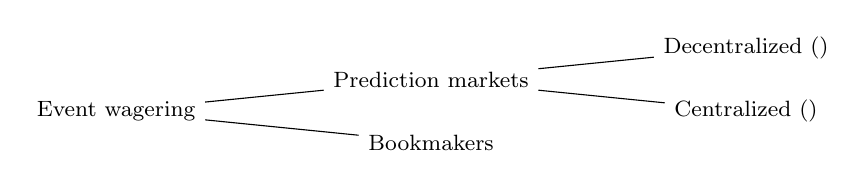
\begin{tikzpicture}[
  font=\footnotesize,
  grow=right,                    % horizontal (left -> right)
  level distance=40mm,           % horizontal gap between levels
  sibling distance=8mm,          % vertical gap between siblings
  box/.style={draw, rounded corners, align=left, inner sep=2pt, text width=28mm}
]
\node{Event wagering}
  child { node{Bookmakers} }
  child { node[]{Prediction markets}
    child { node[]{Centralized (\cepms) } }
    child { node[]{Decentralized (\depms)} }
  };
\end{tikzpicture}

\paragraph{Bookmakers versus prediction markets.}

A wager is a two-party contract with payouts based on the outcome of a future event. Consider Alice and Bob who wager on the same outcome of an event. With a fixed-odds bookmaker (or online betting), Alice's contract is different from Bob's contract in at least two regards: (i) it specifically names Alice as the counterparty and (ii) the payouts could be different if the odds changed between Alice's wager and Bob's. By contrast, in a prediction market contract (called a outcome share), Alice and Bob hold identical contracts: (i) all contracts are between the market operator and whoever redeems the contract, and (ii) the payout is exactly the same (typically \$0 if incorrect and \$1 if correct). Odds are reflected in the price paid for a prediction market contract (\ie variable cost and fixed payout), while a bookmaker contract has a fixed cost and variable payout. Thus the key distinction is that prediction market outcome shares are \textit{fungible} and can be freely traded between participants, enabling a free market that communicates information to the public through outcome share prices, trading volume, market depth, and other financial market metrics. Bookmaking variants, also featuring non-fungible wagers, include pari-mutuel betting, back/lay exchanges, and binary options.

\paragraph{\cepm versus \depm.}

The term \textit{decentralized prediction market} originates from the Ethereum whitepaper~\cite{But13} and we abbreviate it \depm to match terms like DeFi (decentralized finance)~\cite{WPG+22} and DePIN (decentralized physical infrastructure networks)~\cite{LWS+24}. The term \textit{decentralized}~\cite{OKK24} in each of these is actually shorthand for both \textit{decentralized} and \textit{permissionless}, where permissionlessness is generally the more important way \depms distinguish themselves from centralized prediction markets (\cepms). Permissionlessness could extend itself to the market topic, the trading of outcome shares, the closing of the market, and the withdrawing of rewards, but not all systems will open up each of these operations (as we will explain in \S\ref{sec:wf}). We say a system is \depm if at least one is permissionless.

 % = = = = = = = = = = = = = = = = = = = = = = = = = = = = = = = = = = = = = = = = = = = = = = = = 

\subsection{Definitions}
\label{sec:defn}

% !TEX root = ../main.tex

We define a market within a prediction-market system. In contrast to existing definitions, we abstract away details about how they are implemented. If the definitions are not clear, we refer the reader to Appendix~\ref{app:example} where we describe a specific market offered by Polymarket and map each term in the following definitions to this real world example.

\begin{definition}[Market]\label{def:market}
A (single) market is a tuple $M=(E,\Omega,J,R)$, where $E$ is a well-defined uncertain event, $\Omega$ is a nonempty outcome space for $E$, $J$ is a finite index set of contract labels (“shares”), and $R=(R_j)_{j\in J}$ are nonnegative payoff functions with $R_j:\Omega\to\mathbb{R}_{\ge 0}$. When $M$ resolves to $\omega_M\in\Omega$, one unit of share $j\in J$ pays $R_j(\omega_M)$ (in units of $\mathcal{N}$ defined below).
\end{definition}

\begin{definition}[Prediction--market system]\label{def:system}
A prediction--market system is a tuple $\mathcal{S}=(\mathcal{M},\mathcal{N},\mathsf{Res})$, where $\mathcal{M}$ is a countable set of markets, $\mathcal{N}$ is a numeraire (unit of account), and $\mathsf{Res}=\{\mathrm{res}_M\}_{M\in\mathcal{M}}$ is a family of resolution registers such that, for each $M$ with outcome space $\Omega_M$, we have $\mathrm{res}_M\in\{\bot\}\cup\Omega_M$, $\mathrm{res}_M$ is initially $\bot$, and $\mathrm{res}_M$ transitions exactly once to some $\omega_M\in\Omega_M$.
\end{definition}

%\paragraph{Notation (realized outcome).}
%If $\mathrm{res}_M\neq \bot$, define $\omega_M := \mathrm{res}_M\in\Omega_M$.

\paragraph{Remark (Arrow--Debreu Markets).}
For a market $M=(E,\Omega,J,R)$, suppose there exists a bijection $\iota:J\to\Omega$ and
$R_j(\omega)\in\{0,1\}$ with $\sum_{j\in J} R_j(\omega)=1$ for all $\omega\in\Omega$.
Then $M$ is a winner--take--all (Arrow--Debreu) market: a unit claim of label $j$ pays $1$ iff the realized outcome equals $\iota(j)$, and $0$ otherwise.

% = = =


\paragraph{System axioms.}
For every market $M=(E,\Omega,J,R)\in\mathcal{M}$ operating in system $\mathcal{S}=(\mathcal{M},\mathcal{N},\mathsf{Res})$:

\begin{enumerate}
  \item \textbf{Issuance.} The system may increase the outstanding supply of any label $j\in J$ by any $q\ge 0$ subject to policy (unspecified here). Let $S_j(M)\ge 0$ denote the total outstanding supply of label $j$ in $M$.

  \item \textbf{Transfer.} Holdings of each label $j\in J$ are transferable between accounts; transfers conserve per–label totals $S_j(M)$.

  \item \textbf{Burn/Cancel.} The system may decrease $S_j(M)$ via explicit burn/cancel operations according to policy (optionally allowed pre–resolution).

  \item \textbf{Resolution.} The resolution register satisfies $\mathrm{res}_M\in\{\bot\}\cup\Omega$, is initially $\bot$, and transitions exactly once\footnote{Real world \depms like Polymarket might resolve a market, receive a dispute of over the outcome, and resolve it differently after a process (see Section~\ref{wf:close}). In the definition, resolution refers to the final outcome only. An outcome is final when shares can be redeemed for payouts.} to a realized outcome $\omega_M\in\Omega$.

  \item \textbf{Settlement.} Once $\mathrm{res}_M=\omega_M\in\Omega$, any holder of $q$ units of label $j\in J$ may redeem for $q\cdot R_j(\omega_M)$ units of the numeraire $\mathcal{N}$; redeemed units are removed from supply (burned).

  \item \textbf{Conservation of liability.} Let $S_j^{\mathrm{pre}}(M)$ be the outstanding supply of label $j$ immediately before settlement. The total settlement liability is
  \[
    \mathsf{Liability}(M)\;=\;\sum_{j\in J} S_j^{\mathrm{pre}}(M)\, R_j(\omega_M)\;\in\;\mathbb{R}_{\ge 0},
  \]
  which equals the aggregate numeraire paid out if all outstanding units are redeemed.
  
  % Add solvency

  \item \textbf{No pre–resolution obligation.} While $\mathrm{res}_M=\bot$, the system owes no cash payoff on holdings of $(M,j)$ beyond recording balances and permitting issuance/transfer/burn per policy.
\end{enumerate}

% Remark (optional, keep if desired):
% Arrow–Debreu (winner–take–all) markets are obtained by requiring $R_i(\omega)\in\{0,1\}$ and, if desired, $\sum_{i\in I} R_i(\omega)=1$ for all $\omega\in\Omega$.

% = = =






 % = = = = = = = = = = = = = = = = = = = = = = = = = = = = = = = = = = = = = = = = = = = = = = = = 

\newcolumntype{L}[1]{>{\raggedright\arraybackslash}p{#1}} % Fixed-width column

\begin{table}[t!]
\centering
\caption{Over a few days, truthful and untruthful (`cheap talk') evidence was presented to traders. The market reacted to correct signals and effectively filtered out fake signals, demonstrating a beneficial feature of prediction markets.\label{tab:hbo}}
\begin{tabularx}{\textwidth}{|X|L{7cm}|L{1.7cm}|L{1.7cm}|}
\hline
\textbf{Date} & \textbf{Information} & \textbf{Market Impact} & \textbf{Hindsight Verdict} \\
\hline
05 Oct & Partially redacted leaked email from an HBO executive implies Len Sassaman. & Immaterial & Fake \\
\hline
06 Oct & A long-dormant X account belonging to someone who had corrosponded with Sassaman on Twitter posted a new message stating they were interviewed for the documentary. & Immaterial & Fake\\
\hline
07 Oct & Widow of Sassaman states she was not interviewed. & Moderate & Truthful\\
\hline
07 Oct & CNN piece states director `confronts' Satoshi suspect `face-to-face' ruling out Sassaman, David Klieman, and Hal Finney. & Material & Truthful\\
\hline
07 Oct & Samson Mow, featured in the trailer, speculates it will name Adam Back, also featured heavily in the trailer & Material & Wrong but factual basis \\
\hline
07 Oct & End credits of documentary leaked featuring a tribute to Klieman. & Immaterial & Fake \\
\hline
07 Oct & Mow states Nick Szabo refused to discuss with director implying he was not `confronted'. & Material & Truthful \\
\hline
08 Oct & Peter Todd confirms being confronted for documentary but unsure if he will be named. & Material & Truthful \\
\hline
08 Oct & Scene with Todd leaked but inconclusive if it is film's thesis. & Material & Truthful \\
\hline
08 Oct & Commenter on Polymarket claims to screen test and names Nick Szabo. & Immaterial & Fake \\
\hline
08 Oct & Fortune publishes movie review disclosing Todd is named & Very Significant & Truthful \\
\hline
08 Oct & Documentary airs and names Todd & Very Significant & Conclusive \\
\hline
\end{tabularx}
\end{table}

\subsection{An Example of a Market}
\label{sec:hbo}

Before diving deep on the mechanics of decentralized prediction markets, we illustrate how markets work with a lighthearted example. On 3 Oct 2024, a trailer was released with press coverage of a new HBO documentary on Bitcoin to air about a week later on 8 Oct 2024. In an interview, the director stated, the film would question Satoshi's anonymous identity and, `who we land on is unexpected and is going to result in a fair amount of controversy.~\cite{Bec24}' The next day, Polymarket setup a market for speculating on who the documentary would name, providing 15 names plus an `other/multiple' option.\footnote{\polyurl{Who will HBO doc identify as Satoshi?}{https://polymarket.com/event/who-will-hbo-doc-identify-as-satoshi}} A benefit of a decentralized prediction market is allowing niche topics for markets, unlikely to attract mainstream betting websites---in this case, attracting \$44M USD in trading volume. Having an `other' option is also critical after many markets have failed to fully articulate every eventuality and in this case, the winner, was not one of the original 15 names (see Section~\ref{wf:topic}).

In game theory, cheap talk describes strategic misinformation or signalling aimed at shaping beliefs or prices, provided the cost of deception is outweighed by the potential payoff~\cite{CrSo82}. This is well illustrated by what followed in the HBO Satoshi market as new pieces of evidence emerged, some real and some fake, with some fakes relatively elaborate (professional appearing end-credits or hijacking a target's X.com account) as summarized in Table~\ref{tab:hbo}. Further details are provided in Appendix~\ref{app:hbo}.

Also of interest is how the prediction market did not obviously extract insider information which is in violation of what theory would predict~\cite{Han07}. The director did state he did not participate in the market and advised his team working on the film not to either~\cite{Beg24}. Friction for novice users is also perhaps high---web3 apps have a learning curve and if insiders were based in the US, access would require circumvention of Polymarket's geofencing. Perhaps these reasons kept insiders out of the market.

% = = = = = = = = = = = = = = = = = = = = = = = = = = = = = = = = = = = = = = = = = = = = = = = = 

\section{Modular Workflow}
\label{sec:wf}

\begin{center}
\begin{tikzpicture}[
  node distance=0.5cm and 1cm,
  show background rectangle,
  background rectangle/.style={draw, rounded corners, inner sep=6pt}
]

% Top row
\node (infra) {Underlying Infrastructure~\S\ref{wf:chain}};
\node[right=of infra] (topic) {Market Topic~\S\ref{wf:topic}};

% Middle row
\node[below=of infra] (shares) {Share Structure and Pricing~\S\ref{wf:price}};
\node[right=of shares] (trading) {Trading~\S\ref{wf:trade}};

% Bottom row
\node[below=of shares] (resolve) {Market Resolution~\S\ref{wf:close}};
\node[right=of resolve] (settle) {Settlement~\S\ref{wf:clear}};
\node[right=of settle] (archive) {Archiving~\S\ref{wf:archive}};

% Arrows
\draw[->] (infra) -- (topic);
\draw[->] (topic) to[out=-90, in=90, looseness=0.2]  (shares.north);
\draw[->] (shares) -- (trading);
\draw[->] (trading) to[out=-90, in=90, looseness=0.2]  (resolve);
\draw[->] (resolve) -- (settle);
\draw[->] (settle) -- (archive);

\end{tikzpicture}
\end{center}


We now turn to the design landscape of \depms and step through our modular workflow, summarized above. Some design decisions will be common issues for both centralized and decentralized prediction markets. We include these anyways for completeness. However we put the emphasis on discussing design decisions that are pertinent to the decentralization and permissionlessness of prediction markets. 

% = = = = = = = = = = = = = = = = = = = = = = = = = = = = = = = = = = = = = = = = = = = = = = = = 

\subsection{Underlying Infrastructure}
\label{subsec:blockchain_infra}\label{wf:chain}

In theory, a decentralized and permissionless system might run on a system other than a blockchain, but blockchain technology underlays all known \depms. Selecting a blockchain constitutes the initial design decision within our modular workflow. In selecting a blockchain, a set of desirable features include expressive smart contracts, low transactions fees, fast finality, guaranteed inclusion, and censorship resistance. The earliest research was in agreement that Bitcoin Script was not powerful enough to operate a \depm, and a separate chain (perhaps integrated with Bitcoin as a sidechain) would be required. Later Ethereum was deployed, providing general smart contracts, and most \depm activity moved to it. Much later, high fees on Ethereum caused the diversification of the VM-based blockchain space into numerous competing chains and layer 2 (L2) scalability solutions. As of today, the most active \depms run on chains built to execute smart contracts (\eg EVM or WASM). Most no longer run on Ethereum but on either an Ethereum competitor (\eg Polygon or Solana) or an Ethereum L2 (\eg Arbitrum or Optimism).

Generally, there are no strong qualitative differences between the named blockchain options---it is a choice driven by fees, user base, and supporting infrastructure. In all cases, the logic of the prediction market operations is placed in smart contracts and the blockchain executes the contracts. A materially different approach is  to put the prediction market logic into the blockchain rules themselves, either with a purpose-built blockchain or with a customized layer (called an L3) that uses custom rules but settles on a standard L1 or L2.

%MEV?

%Non-blockchain

% = = = = = = = = = = = = = = = = = = = = = = = = = = = = = = = = = = = = = = = = = = = = = = = = 

\subsection{Market Topic}\label{wf:topic}

\cepms include the Iowa Electronic Markets, Kalshi, and PredictIt, as well as InTrade historically. These systems exercise control over what topics may form a market and thus are \textit{permissioned} with respect to market topics. They also operate under regulations that may restrict markets to certain topics or fully ban operations in regulated jurisdictions~\cite{Du19}. 

By contrast, \depms like Augur, Gnosis, and PlotX enable \textit{permissionless} market creation by any user without centralized review. This removes the regulatory hook, enables niche topics that might not attract mainstream interest, and allows markets to be created without delay after real world events. However it can also lead to a greater incidence of malformed (or even malicious) market definitions, and unlawful topics, such as the `assassination markets' which appeared on Augur in 2018. \depms are generally web3 applications which means that a web-based user interface mediates transactions between the user and the underlying smart contracts. Market topic moderation could be implemented at the web3 layer (\eg Predictions.Global unlisted assignations markets from Augur's smart contracts) but this does not prevent users from building an alternative UI or directly transacting with the smart contracts. While \depms have the option to operate permissionlessly, they may also choose to permission market creation while leaving other aspects permissionless. At the time of writing, Polymarket is considered a \depm and while market topics can be suggested by users, final approval is made by a Market Integrity Committee~\cite{ClEsGS21}.

A \textit{hybrid model} puts some controls on topic creation without centralizing it fully. For example, proposers may have to stake tokens to propose a market, and while the market is optimistically published, a review (either centralized or via an on-chain voting mechanism) could remove the market and/or slash the proposer.  


% !TEX root = ../main.tex

% = = =

\begin{table}[t!]

\caption{Some pitfalls that illustrate the difficulty in properly defining a prediction market topic. \label{tab:pitfalls}}

\begin{tabular}{L{0.2\textwidth} L{0.8\textwidth}}
\hline
\textbf{Pitfall} & \textbf{Description} \\
\hline

% = = =

\multirow{2}{\linewidth}{Borderline Categories}
  & \textit{Example}: A market on whether Zelensky would wear a suit was contested when he wore a single-breasted jacket with patch chest pockets and matching trousers;\tablefootnote{\polyurl{Will Zelenskyy wear a suit before July?}{https://polymarket.com/event/will-zelenskyy-wear-a-suit-before-july}} media equivocated on describing it as a suit.\tablefootnote{Google Docs: \href{https://docs.google.com/document/d/1p0CSpse6YwLApvwKt173bDg1cQVNcNEe0_2sNCvhaZs/}{Did President Zelenskyy wear a suit before July 2025?}.} \\ \cline{2-2}
  & \textit{Mitigation}: Clearly state inclusion/exclusion criteria (\eg a subsequent market on a potential hug between Trump and Putin spent a paragraph defining a hug.\tablefootnote{\polyurl{Will Trump and Putin hug on Friday?}{https://polymarket.com/event/will-donald-trump-and-vladimir-putin-hug-on-friday}}) \\ \hline
  
  % = = =

\multirow{2}{\linewidth}{Precedence Gaps}
  & \textit{Example}: A proposition bet on the colour of the 2014 Super Bowl  `Gatorade shower' was contested when the coach was showered twice with different colours~\cite{BCFKMN14}. A market on whether Zelensky would be `the' 2022 TIME Person of the Year was contested when both Zelensky and the Spirit of Ukraine were named.\tablefootnote{\polyurl{Will Volodymyr Zelenskyy be the 2022 TIME Person of the Year?}{https://polymarket.com/event/will-volodymyr-zelenskyy-be-the-2022-time-person-of-the-year}} \\ \cline{2-2}
  & \textit{Mitigation}: Parse the predicate for any statements needing explicit precedence (\eg first, majority, primary); or establish a payout rule for ties; or include an outcome for `multiple.' \\ \hline

% = = =

\multirow{2}{\linewidth}{Hidden Presumptions}
  & \textit{Example}: A market concerning a divorce presumes the couple are married (as opposed to common law) which was unknown.\tablefootnote{\polyurl{Astronomer Divorce Parlay}{https://polymarket.com/event/astronomer-divorce-parlay}} \\ \cline{2-2}
  & \textit{Mitigation}: Parse the predicate for any presumptive statements and remove/address them.\\ \hline

% = = =

\multirow{2}{\linewidth}{No Ground Truth}
  & \textit{Example}: A market on whether a US strike destroyed an Iranian nuclear facility was contested when each country reported different outcomes and no neutral third party was granted access to the site.\tablefootnote{\polyurl{Fordow nuclear facility destroyed before July?}{https://polymarket.com/event/fordow-nuclear-facility-destroyed-before-july}} A market on whether Baron Trump was `involved' in the \$DJT memecoin lacked an authoritative source.\tablefootnote{\polyurl{Was Barron involved in \$DJT?}{https://polymarket.com/event/was-barron-involved-in-djt}} An election market on Venezuela's president was contested when the government declared Maduro won, while international media and democracy watchdogs declared Gonzalez received more votes.\tablefootnote{\polyurl{Venezuela Presidential Election Winner}{https://polymarket.com/event/venezuela-election-winner}} \\ \cline{2-2}
  & \textit{Mitigation}: Avoid markets without ground truth sources; or include an additional option in the market for unverified. \\ \hline

% = = =

\multirow{2}{\linewidth}{Platform Coupling}
  & \textit{Example}: Hypothetically, traders who correctly predict USDC will completely de-peg on a platform that pays out in USDC will receive a payout but it will be worthless (\cf~\cite{BCFKMN14}). \\ \cline{2-2}
  & \textit{Mitigation}: Avoid markets that are self-referential, including topics on the platform itself and its numinaire. \\ \hline

% = = =

\end{tabular}
\end{table}

% = = =

Careful attention must be paid to both the general topic of the market and the `fine-print' or exact predicate that decides the market. Table~\ref{tab:pitfalls} provides several examples of pitfalls. A pitfall in the predicate means the market topic is acceptable but there is an issue with its exact specification (\eg a market about wearing a suit needs to define a suit). A pitfall in the topic means the topic itself is problematic, even if it is worded impeccably (\eg a Polymarket market about whether Polymarket will shut down is problematic because winners will not be paid if it does). The first pitfall, borderline categories, is very prominent with many other disputes, including whether enforcement against TikTok in the US constitutes a ban,\footnote{\polyurl{TikTok banned in the US before May 2025?}{https://polymarket.com/event/tiktok-banned-in-the-us-before-may-2025}} or if finding debris from the Titan submersible constitutes it being found.\footnote{\polyurl{Will the missing submarine be found by June 23?}{https://polymarket.com/event/will-the-missing-submarine-be-found-by-june-23}} 

These issues are not limited to \depms and apply to event wagering in general, however some issues are more pronounced in \depms. If market creation is permissionless, market creators may be amateurs and error-prone; may draft adversarial markets to trick traders; or duplicate existing markets, thinning out liquidity. \cepms have the latitude to organize, pause, or revise markets or ban users. \depms may give themselves this latitude at the risk of appearing less permissionless. Further it seems inevitable that some markets will fall into a pitfall and \depms have to carefully consider how dispute resolution will work while also appealing to blockchain enthusiasts.

Dealing with definitional pitfalls has been, to date, a trial and error process where market creators learn from past mistakes and ad hoc `legalese' (e.g., a `consensus of credible reporting' may be used to resolve markets) is copied from market to market. Future research could develop machine-checkable predicate specifications (precedence rules, ranked sources, time semantics, and default outcomes) and verify they are well-defined with model checking. 

If issues in a market's topic or definition are uncovered while the market is still active, \depms like Polymarket allow `additional context' notes to be added. However these clarifications could alter the market ex post and also disadvantage traders who do not see the note. The latter can be mitigated by advertising that a note will be published, always publishing at the same time (\eg 5pm ET), and clearing standing limit orders from an orderbook before posting.

% = = = = = = = = = = = = = = = = = = = = = = = = = = = = = = = = = = = = = = = = = = = = = = = = 

\subsection{Share Structure and Pricing}\label{wf:mech}\label{wf:price}

The core requirement of a prediction market is that wagers are represented by fungible outcome shares. The structure of outcome shares typically falls into one of three categories and two variants (although more exotic structures are possible and explored in research). Consider a market with three possible outcomes: $\Omega=\{\mathsf{A}, \mathsf{B}, \mathsf{C}\}$. 

The first structure we term \textit{winner-take-all (WTA)} and is prominent on Iowa Electronic Markets and supported by Augur and Gnosis. A WTA market issues a outcome share for each outcome $J=\{j_\mathsf{A}, j_\mathsf{B}, j_\mathsf{C}\}$. If the outcome is $\mathsf{B}$, the share $j_\mathsf{B}$ pays \$1 (or one unit of numeraire $\mathcal{N}$) and the other shares pay \$0. For any $k\in\{\mathsf{A},\mathsf{B},\mathsf{C}\}$,

\[R_{j_{\mathsf{k}}}(\omega)=\begin{cases}1, & \text{if } \omega=\mathsf{k},\\0, & \text{otherwise.}\end{cases}\]

For a WTA market to be well-functioning, conditions must hold on outcome shares. (i) They should be \textit{mutually exclusive} so no more than one share wins: $R_{j_{\mathsf{k}}}(\omega)R_{j_{\mathsf{\ell}}}(\omega)=0 \quad \forall\omega\in\Omega, \forall\mathsf{k}\neq\mathsf{\ell} $; and (ii) they should be \textit{complete} so at least one share wins: $\sum_{\mathsf{k}\in\Omega} R_{j_{\mathsf{k}}}(\omega)=1\quad \forall \omega\in\Omega$. If they are not mutually exclusive, the operator could be undercollateralized for making all payments. If they are incomplete, a deficient market might end with all participants receiving \$0. A consequence is that holding one share for each outcome is equivalent to holding \$1, a fact we will return to in the next section on trading. 

In a WTA market, the price of a outcome share (\eg $p(j_\mathsf{A})=\$0.54$) is a proxy for the probability that the outcome will occur (\eg $\mathrm{Pr}[\omega=\mathsf{A}]=54\%$). A common adage is the prices of each share sum to \$1.00 ignoring fees and discounting (\eg $p(j_\mathsf{A})=\$0.54$, $p(j_\mathsf{B})=\$0.23$, $p(j_\mathsf{C})=\$0.23$) but this is imprecise. Outcome shares (like anything) have two prices: a bid price (what a trader is willing to buy for) and an ask price (willing to sell for). If the sum of the bid prices exceeds \$1.00 or if the sum of ask prices are below \$1.00, arbitrageurs have an opportunity to secure risk-free profit through a trade that will erase the condition when fully extracted. This means the sum of bids and sum of asks should result in the bid-ask spread straddling \$1.00 but the amount of the spread could be arbitrarily large. So in user interfaces that display a single `price' (\eg the last sale price or the midpoint between the best bid and the best ask), prices may indeed not sum to \$1.00---this is not a market failure, just a misunderstanding.  

 % = = =
 
The second structure we term a \textit{yes-no bundle (YNB)}. YNB markets were prominent on InTrade and are currently prominent on Polymarket. A YNB market issues two outcome shares for each outcome, a `yes' and a `no:'  $J=\{j_{\mathsf{A_Y}}, j_{\mathsf{A_N}}, j_{\mathsf{B_Y}}, j_{\mathsf{B_N}}, j_{\mathsf{C_Y}},j_{\mathsf{C_N}} \}$. For any $k\in\{\mathsf{A},\mathsf{B},\mathsf{C}\}$,

\[
R_{j_{\mathsf{k_Y}}}(\omega)=
\begin{cases}
1, & \text{if } \omega=\mathsf{k},\\
0, & \text{otherwise.}
\end{cases}
\qquad
R_{j_{\mathsf{k_N}}}(\omega)=
\begin{cases}
1, & \text{if } \omega\neq\mathsf{k},\\
0, & \text{otherwise.}
\end{cases}
\]

Each outcome-specific pair $\{j_{\mathsf{k_Y}}, j_{\mathsf{k_N}}\}$ constitutes a two-outcome WTA market ($\mathsf{k}$ vs.\ not-$\mathsf{k}$). A YNB market is the union of these pairs, so the WTA exclusivity and completeness properties hold per pair. However exclusivity and completeness do not necessarily hold across all bundles, allowing more flexible markets. For example, a market on what words Trump will say in a congressional address included Bitcoin (no), beautiful at least 10 times (yes), and Canada (yes).\footnote{\polyurl{What will Trump say during address to Congress?}{https://polymarket.com/event/what-will-trump-say-during-state-of-the-union?tid=1755462445353}} Multiple words can resolve to yes (not exclusive) and it is possible he says none of the listed words (not complete). If a YNB market is established and being actively traded, because it is not complete, new outcomes can be added fairly to the market mid-flight. 

A variant of the YNB market is one where, even though it is not necessary, the yes share outcomes are in fact complete and exclusive. In other words, each yes/no bundle is a WTA market and the set of all yes shares is also a WTA market. We term this variant as \textit{YNB negative risk (YNB-NR)}, a term introduced by Polymarket. Recall that in a WTA market, roughly speaking, the share prices sum to \$1 (modulo the fine print about bid/ask spreads above). For a YNB-NR market, the Yes shares are the same as a WTA share and sum to \$1, while the No shares will sum to $|\Omega|-1$. The Satoshi/HBO YNB market from Section~\ref{sec:hbo} was made exclusive and complete across bundles by including a bundle for the outcome: `other/multiple.' 

Further, in a YNB market, holding a No outcome share for Hal Finney has the same payoff as holding a Yes share for every other candidate. Polymarket introduced a \textit{negRisk} gadget that allows a trader to convert any No share into a portfolio of Yes shares for every other outcome. This enables traders to adjust their positions with less buying/selling on the markets, and also aligns prices between Yes and No markets with low friction arbitrage opportunities. Formally, a single No share has the equivalence (\ie same payoff ignoring fees and discounting):

\[
j_{\mathsf{k_N}} \equiv \sum_{\ell \in \Omega\setminus\{\mathsf{k}\}} j_{\mathsf{\ell_Y}} \quad\text{for any }\mathsf{k}\in\Omega.
\]

And multiple No outcome shares can be converted into Yes shares plus cash:

\[
\sum_{\ell \in \Omega\setminus\{\mathsf{k}\}} j_{\mathsf{\ell_N}}
\equiv
j_{\mathsf{k_Y}} + \$1\cdot(|\Omega|-2)
\]

% = = = 

The third structure is a market where the outcome is a quantity of interest (\eg popular vote, temperature, price level, \etc) observed at a cutoff time. Termed a \textit{linear} or \textit{scalar} market, there is only one share and its payout is what value the quantity takes on (perhaps normalized to the range $[0,1]$ with rounding). As an example, in a market on Trump's popular vote, if the quantity is 49.8\%, the share will pay \$0.498. Shares can also be sold in bundles with `long' receiving \$0.498 and `short' receiving (\$1-\$0.498).

Formally, if we let $X:\Omega\to\mathbb{R}$ be the observed quantity, and $[a,b]$ be an interval of values, then the linear outcome share $j_{\mathrm{lin}}$ pays:

\[
R_{j_{\mathrm{lin}}}(\omega)=
\begin{cases}
0, & X(\omega)\le a,\\[3pt]
\dfrac{X(\omega)-a}{\,b-a\,}, & a< X(\omega) < b,\\[6pt]
1, & X(\omega)\ge b.
\end{cases}
\]

While linear markets are supported by \depms like Augur, Gnosis, and Omen, they are not frequently used. Even though Polymarket uses the Gnosis Conditional Tokens Framework (CTF) which supports linear markets, it instead approximates one by splitting the quantity into `buckets' and running a YNB market for each bucket. This allows greater code-reuse and possibly avoids small edge cases over the exact resolution of the quantity (\eg off by 0.1 percentage disputes). However a problem with buckets is as follows: Alice estimates correctly that Trump will win the election with 49--51\% of the popular vote. If there is a bucket for 45--49.9\% and a bucket for 50--54.9\%, Alice's forecast does not fit into a single bucket. Generally, an unfortunate cutpoint between boundaries can dilute expected return on capital (as investors buy more than one bucket) and can lead to volatile market jumps when the market forecast switches between buckets.\footnote{\polyurl{April 2025 Temperature Increase (ºC)}{https://polymarket.com/event/april-2025-temperature-increase-c4}} 

% = = = = = = = = = = = = = = = = = = = = = = = = = = = = = = = = = = = = = = = = = = = = = = = = 

\subsection{Trading}\label{wf:trade}
% JC

A near universal difference between any \cepm and \depm is that a \depm allows outcome shares to be withdrawn from the platform, typically in a form compliant with a token standard such as ERC-1155. By contrast, \cepm outcome shares are held in-house by the operator. Withdrawing outcome shares allows traders to exchange tokens outside of the platform and to compose with third party DeFi services (\eg on-chain trading, lending, leverage, \etc). From a software development perspective, it also means that \depms can be built with external libraries or using outside infrastructure.  Options for trading outcome shares can be broken into two steps: (i) how does the first outcome share come into existence and how does the first trader trade, and (ii) how do traders trade once a market has been established? 

\subsubsection{The first trade.} Probably the greatest evolution in \depms, from Truthcoin through Augur and Gnosis to Polymarket, concerns how the first trade happens. There are three options: \textit{automated bookmaking}, \textit{splitting}, and \textit{matching}. \textit{Automated bookmaking} was popularized through the academic work of Robin Hanson and was first suggested for \depms by Truthcoin, which heavily influenced Augur and Gnosis. In this model, the operator sets initial prices for each outcome share (equivalent to setting market odds) and collateralizes enough payout money to cover a worst-case loss. If Alice is the first trader, she can immediately trade with the operator. The operator is autonomous and sets buy/sell prices algorithmically, originally using Hanson's logarithmic market scoring rule (LMSR). The key point is that the operator is Alice's counterparty; if Alice wins, the operator loses, and vice-versa. The pros are instant liquidity for the first trader and the cons are risk of losing money and the burden of needing to set initial odds (getting them wrong increases the chances it loses). Acute readers might wonder if this is the same as an automated market maker (\eg Uniswap) discussed below. Roughly speaking, a WTA market run by automated bookmaking is termed a cost-function prediction market (CFPM) and a CFPM is equivalent in pricing (and trade costs) to an AMM (defined by a set of axioms) with the right invariant.

The second approach, \textit{splitting}, is used by IEM and was first suggested for \depms by the Princeton \depm. Augur switched to this approach, Gnosis implemented it in CTF, and Polymarket uses it. Recall that in a WTA market, exactly one share in a set of shares will payout \$1. This means that holding a complete portfolio of every share is equivalent (in payoff, ignoring fees and discounting) to holding \$1. Splitting allows any trader to purchase a complete portfolio of shares for \$1 (and generally \textit{merging} is also permitted where a complete set can be redeemed for \$1 at any time before the market closes). Alice can obtain a set of shares and list asking prices (through a limit order book or by being the first liquidity provider in an AMM) for some or all of the shares, and if Bob is willing to buy a share from Alice, the first trade occurs. The pros to splitting is that the operator has zero exposure to the market, and the operator is always fully solvent, while the con is that Alice must wait for a second trader, Bob, before she can trade. 

In YNB markets, each outcome’s YES/NO pair is its own two-outcome WTA market. Splitting is per outcome: converting \$1 of collateral mints one \(j_{\mathsf{k_Y}}\) and one \(j_{\mathsf{k_N}}\) for the chosen \(\mathsf{k}\). Hence, within any bundle \(\mathrm{totSupply}(j_{\mathsf{k_Y}})=\mathrm{totSupply}(j_{\mathsf{k_N}})\). Across outcomes, however, supplies are uncoupled—the total minted for the \(\mathsf{A}\) bundle need not match that for \(\mathsf{B}\) or \(\mathsf{C}\).

The third approach, \textit{matching}, was used by InTrade and a variant by Fairlay. Briefly, it mirrors a futures market, where Alice posts a desired short/long position at a chosen price on an orderbook with a margin account holding enough cash to cover her maximum loss if she obtains the position. If Bob is willing to take the other side, also with sufficient margin for his maximum loss, the operator matches them, creates two shares and gives them to Alice and Bob. Alice and Bob are not counterparties, both settle with the operator once the shares are created, however their coincidence of wants (COW) is necessary for the operator to create shares at no risk to itself. The pros/cons mirror those of splitting but matching is operationally more complex: the operator needs to run an orderbook and is involved in the trading process. 

\subsubsection{Trading in established markets.}

Once outcome shares are in wide circulation, they can be traded any way fungible blockchain tokens can be traded. This includes \textit{centralized exchanges} that custody the tokens and use central order book (CLOBs); \textit{partially decentralized exchanges} where CLOB matching is done off-chain and settlement is done on-chain; or \textit{fully on-chain exchanges}, of which automated market makers (AMMs) are the most common. 

Of interest, AMMs were born out of Gnosis' research into automated bookmarking for prediction markets. They first developed alternatives to the LMSR rule, including the constant product rule. Initially, it was proposed that a trader holding two kinds of tokens could set up an automated market maker using this, or other, rules. This is precisely what the prediction market operator does in automated bookmaking. In parallel, Bancor worked on exchanges where multiple traders could contribute tokens to a common liquidity pool. Uniswap v1 merged these two ideas to create the basic template of an AMM that is common today.

Despite the direct lineage between prediction markets and AMMs, AMMs are problematic for prediction market trading. \depm outcome shares behave in specific ways that differ from typical crypto-assets and tokens. The price is strictly bounded between \$0 and \$1, the value of a share can jump to \$0 or \$1 near-instantly when an event outcome is finalized, and once finalized, the price is permanent. When real world events occur, AMMs can be drained faster than liquidity providers can withdraw liquidity. Adapting AMMs to these constraints is an interesting open problem. Paradigm’s pm-AMM tapers liquidity as a scheduled expiry approaches, which helps for events with a known horizon; but many markets jump or resolve unexpectedly, so pre-expiry shocks can still hurt liquidity providers.

When trading on-chain, miners and other users can front-run transactions, an area of study called maximum extracted value (MEV). Although the term MEV did not exist at the time, the Princeton \depm describes the MEV problem extensively and proposes a mitigation now called a frequent batch auction (FBA) (again, the term FBA was not popularized until later) to be conducted at the blockchain-level (adaptable to a layer 3 chain). On-chain FBAs have been studied and while linear time operations in the size of the orderbook are still infeasible for Ethereum or even layer 2 roll-ups, succinct proofs that auctions were closed correctly could be used.  

A final trading-relevant subject for prediction markets is arbitrage. Arbitrageurs ensure market prices are consistent, for example across all shares in a WTA market or between Yes/No bundles in a YNB market. A recent paper studies combinatorial arbitrage on Polymarket between markets with logically related predicates (\eg Republicans win the presidency; Trump wins the presidency) and measures roughly \$40M USD of realized arbitrage profits over the measurement period. 

% = = = = = = = = = = = = = = = = = = = = = = = = = = = = = = = = = = = = = = = = = = = = = = = = 

\subsection{Market Resolution}\label{wf:close}

It is possible that a market topic can be determined on-chain (\eg total value locked in a DeFi service) in which case resolution is simple, however typically, prediction market outcomes concern facts that are off-chain. In these cases, resolution is the process of finalizing an off-chain outcome in an on-chain market. The predominate approaches are the following: self-settling markets, auto-resolve rules, using a designated arbiter, using a network of reporters, and crowdsourcing a vote. The term \textit{oracle} is commonly used for any of the latter three approaches (while the first two could be considered oracle-less). A \depm may use a hybrid approach. For example, an arbiter might optimistically resolve a market outcome while also allowing disputes. If an outcome is disputed, it is escalated to a crowdsourced vote. If the vote is considered defective, a further escalation could allow an Admin account to overrule the decision. The ultimate backstop is the law which would not stop a wrong outcome but could be used to remunerate parties damaged by it.

Oracle-less approaches are largely academic. A \textit{self-settling market} assumes \textit{splitting} and \textit{merging} (see \S\ref{wf:trade}) of shares and relies on participants with winning shares to purchase the losing shares (for close to \$0) and redeem \$1 by merging them. If losing shares do not trade near \$0 or become illiquid, the broader market might accept winning shares as a substitute for dollars. If a market outcome is contentious with no recognized winner (\eg a poorly defined market in \S\ref{wf:topic}), the market will not settle. An \textit{auto-resolve rule} could also be used such that outcomes are finalized when their token trades above \$0.99 for at least $t$ time. Auto-resolve rules are subject to market manipulation (losing shares are wash traded near \$1 long enough to finalize, in which case they are worth \$1) or griefing attacks (yes shares are traded below \$0.99 to prevent finalization). 



% https://augur.mystrikingly.com/blog/scaling-augur-part-2-a-roadmap#:~:text=An%20interesting%20idea%20would%20be,for%20resolving%20without%20your%20aid


The \textit{designated arbiter} space is evolving, with platforms exploring a shift from centralized human arbiters to AI councils. Kalshi exemplifies centralized resolution: staff settle markets per published rules/sources; as a CFTC-regulated DCM and for platform credibility, team is incentivized to resolve accurately.[https://www.cftc.gov/PressRoom/PressReleases/8302-20], [https://help.kalshi.com/markets/markets-101/market-rules]
Chaos Labs’ Edge Proofs is a concrete AI-arbiter design where a decentralized network of agents from multiple models gather evidence from predeclared sources and finalize only on a consensus threshold. [https://chaoslabs.xyz/posts/edge-proofs-ai-powered-prediction-market-oracles] [https://blog.langchain.com/how-chaos-labs-built-a-multi-agent-system-for-resolution-in-prediction-markets/]
Because AI is probabilistic and blockchains are deterministic, no-consensus loops can arise; timebox decisions and fall back (relax threshold, resolve Unknown, or escalate, e.g., to UMA). AI oracles also inherit adversarial ML risks [https://www.arxiv.org/pdf/2507.02125] such as RAG poisoning [https://arxiv.org/html/2402.07867v1] Blockchain has seen analogous integrity failures with mutable off-chain references (e.g., Marlinspike’s “poop-emoji” NFT [https://moxie.org/2022/01/07/web3-first-impressions.html]).
Early empirical results are mixed but promising: a Chainlink study of 1,660 Polymarket questions reports ~89.3\% accuracy (sports 99.7\%, politics 84.3\%) with temporal-reasoning challenges.[https://blog.chain.link/ai-oracles/]

% https://www.lesswrong.com/posts/tJmpsEevCcEfL6a7Z/self-resolving-prediction-markets

%  final authority is a specific signing address; behind this address could be a trusted organization (\eg AP via Everipedia OraQles\footnote{Etherscan: \url{https://etherscan.io/address/0x0792724900B551d200D954a5Ed709d9514d73A9F}}) 



\textit{Reporter networks} deliver fast, parameterizable, and auditable resolution for markets tied to structured external data (prices, scores). An aggregation contract (e.g., a Chainlink feed) acts as the definitive on-chain authority. Multiple independent reporters submit signed observations off-chain; an off‑chain consensus protocol (OCR) coalesces these into a single report whose value is typically the median (or a mean with outlier filtering) and whose metadata (round ID, timestamp) and quorum signatures are verified on-chain. Updates are emitted when deviation or heartbeat thresholds are met, giving explicit control over latency/recency and bounding staleness under network stress. Median aggregation is resilient to a minority of faulty or adversarial reporters (Byzantine tolerance), while source and operator diversity mitigate data‑correlation risk; compressing n submissions into one update reduces gas and surface area. The result is a deterministic, publicly auditable outcome primitive: DePM contracts read the aggregator at resolution time and settle without discretionary intervention.

Thales and its Overtime on‑chain sportsbook instantiate this model end‑to‑end: market predicates reference Chainlink sports feeds for scores and final results, odds can be parameterized from on‑chain feeds, and expiry reads the aggregator’s answer to resolve. Augur Turbo similarly relies on reporter‑network feeds for schedules, scores and stats, so sports markets settle immediately upon event close. Entropyfi resolves scalar price rounds by sampling Chainlink aggregator contracts at round start/end and uses on‑chain automation (Keepers) to trigger settlement, coupling reporter‑network data with deterministic payout logic. 

% SKC paper:  Srinivasan, Karger, and Chen (2023) 




In \textit{crowdsource voting} systems, final authority rests with an on-chain arbitrator whose outcome is chosen by stake-weighted voting; the system finalizes to the majority of stake, which does not guarantee resolution to the real outcome. There are two designs: (i) Schelling/always-vote (e.g., Augur/REP), where token holders stake and vote on every market and repeated disputes can escalate to a fork lasting up to 60 days—effectively pausing other non-finalized markets while REP holders migrate to a “true” universe—making this approach slow and operationally heavy, [https://ar5iv.labs.arxiv.org/html/1501.01042] and (ii) optimistic, dispute-driven, where anyone proposes an answer with a bond, the market resolves if unchallenged during liveness, and only disputed cases go to a vote— UMA is the canonical version (on Polymarket: ~2-hour challenge window, ~\$750 bond, and a DVM commit–reveal vote if challenged). This optimistic pattern is faster and more cost-effective because unchallenged proposals finalize after a short liveness period and only disputes are escalated to the DVM, avoiding the cost and delay of global voting.
[https://docs.uma.xyz/protocol-overview/how-does-umas-oracle-work]
[https://docs.polymarket.com/developers/resolution/UMA]
A closely related optimistic stack is Reality.eth + Kleros, where disputed questions go to a randomly drawn, staked juror court that uses commit–reveal; jurors in the majority are rewarded while those in the minority are penalized. [https://kleros.io/whitepaper.pdf]
Token-voted decentralizes market resolution but inherits governance voting’s flaws and adds carrot/stick incentives that reward the eventual majority while penalizing minorities and non-participants Token-voted dispute resolution decentralizes market resolution but inherits governance voting’s flaws and adds carrot/stick incentives that reward the eventual majority while penalizing minorities and non-participants. In practice, stake can centralize, enabling whale capture: a coordinated or whale-tilted majority can settle a market incorrectly with no penalty to itself—only the minority is slashed—mirroring patterns seen in governance (e.g., Uniswap, where 11 wallets can determine a majority; a16z’s influence on a proposal) [https://www.sciencedirect.com/science/article/pii/S2096720924000216], [https://cointelegraph.com/news/a16z-votes-against-proposal-to-deploy-uniswap-v3-on-bnb-chain] A similar concentration risk surfaced on Polymarket/UMA during a governance attack [https://www.coindesk.com/markets/2025/03/26/polymarket-suffers-uma-governance-attack-after-rouge-actor-becomes-top-5-token-staker]. For UMA specifically, the top five wallets control ~45.6\% of votes and the top 13 exceed 65\%, enough to meet the passing threshold
[https://dune.com/uma\_protocol/uma-protocol]
These payoff asymmetries induce “beauty-contest” behavior: because minorities are slashed and majorities paid, rational voters may try to forecast the majority rather than report private information, permitting majority-wrong outcomes when expectations align or large holders coordinate. Finally, bribery and vote-buying (the $p+\epsilon $ attack) can flip results whenever an attacker’s external payoff from a wrong resolution exceeds the system’s economic security [https://blog.ethereum.org/2015/01/28/p-epsilon-attack]
Beyond capture and bribery, token voting can impose real costs when platform policy diverges from oracle outcomes. In June 2024, UMA voters resolved “No” on a high-profile Polymarket market, while Polymarket publicly deemed the opposite “conclusive” and refunded users—an unusual split that highlights governance/interpretation friction between platform administrators and token-vote results
[https://www.coindesk.com/markets/2024/06/27/polymarket-contradicts-its-oracle-service-in-rarity-for-prediction-market?](https://www.coindesk.com/markets/2024/06/27/polymarket-contradicts-its-oracle-service-in-rarity-for-prediction-market)]
As a possible mitigation, platforms like Polymarket that rely on UMA’s token-vote oracle could, in theory, replace it with a native dispute token, leveraging their scale to increase economic security and align incentives for truthful voting and platform integrity by directing a share of platform revenues to voters.
Kleros addresses several of these challenges by using commit–reveal to prevent mid-round copycatting, an appeal ladder that roughly doubles the jury (+1) and increases fees at each step to make capture and bribery costlier, and topical subcourts so disputes are heard by more knowledgeable jurors.

A similar concentration risk surfaced on Polymarket/UMA during a governance attack [7].

For UMA specifically, the top five wallets control ~45.6\% of votes and the top 13 exceed 65\%, enough to meet the passing threshold [8]
These payoff asymmetries induce “beauty-contest” behavior: because minorities are slashed and majorities paid, rational voters may try to forecast the majority rather than report private information, permitting majority-wrong outcomes when expectations align or large holders coordinate. Finally, bribery and vote-buying (the p+$\epsilon$ attack) can flip results whenever an attacker’s external payoff from a wrong resolution exceeds the system’s economic security [9]
Beyond capture and bribery, token voting can impose real costs when platform policy diverges from oracle outcomes. In June 2024, UMA voters resolved “No” on a high-profile Polymarket market, while Polymarket publicly deemed the opposite “conclusive” and refunded users, an unusual split that highlights governance/interpretation friction between platform administrators and token-vote results [10]
As a possible mitigation, platforms like Polymarket that rely on UMA’s token-vote oracle could, in theory, replace it with a native dispute token, leveraging their scale to increase economic security and align incentives for truthful voting and platform integrity by directing a share of platform revenues to voters.
Kleros addresses several of these challenges by using commit–reveal to prevent mid-round copycatting, an appeal ladder that roughly doubles the jury (+1) and increases fees at each step to make capture and bribery costlier, and topical subcourts so disputes are heard by more knowledgeable jurors.



% = = = = = = = = = = = = = = = = = = = = = = = = = = = = = = = = = = = = = = = = = = = = = = = = 

\subsection{Settlement}\label{wf:clear}

The slogan `sweat the game, not the payout' is used to differentiate regulated sportsbook operators from `neighbourhood bookies,' however even legitimate operators in the US have allegedly denied payouts using a legal loophole.\footnote{A law protects sports books from obvious errors, like a `fat finger' when setting odds, but can be misused to claim long-shot bets were `obvious mistakes' after the fact.} The advantage of a \depm in this context is two-fold: (i) payouts are fully (or largely) autonomous, not subject to human discretion, and (ii) the share structure ensures the operator has zero risk (or predetermined bounded risk, in the case of automated bookmaking) and is therefore financially indifferent to making any fair payout (see Axioms in Section~\ref{sec:defn}).

%	5.	Collateral \& solvency.
%Prove on-chain that total liabilities ≤ locked collateral; prefer stable collateral for event risk.
%• Polymarket/Omen: USDC-style stablecoins; CTF algebra guarantees solvency on split/merge.
%• Augur: historically ETH/DAI; solvency via complete-set mint/burn.

Once the market is resolved, a \depm will enable each winning share to be converted into 1 unit of the numeraire (\eg 1 USD in a stablecoin) and transferred into the user's self-custody. While a \depm in theory could \textit{push} payouts to users, it is common to wait for the user to initiate the redemption. Augur, CTF, and Omen implement such a \textit{pull} mechanism. In this case, users pay the gas cost of the redemption which requires users to hold the native currency of the underlying blockchain. Polymarket offers gasless withdrawals (using OpenGSN relayers), however users can bypass this at their choice. In a pull model, some users may not redeem their shares in a timely manner---a \depm may opt to sweep this surplus into its own capital or burn it, but \depms generally hold it on-chain in perpetuity. As with any smart contract allowing withdraws based account balances, hardening against reentrancy attacks is critical.


% = = = = = = = = = = = = = = = = = = = = = = = = = = = = = = = = = = = = = = = = = = = = = = = = 

\subsection{Archiving}\label{wf:archive}

Publicly accessible \depm data provides society with a useful forecasting tool, and archival datasets enable calibration, insight into historical events, and replication of findings. On-chain records (state, logs, and calldata) inherit strong archival and verification properties so long as the chain persists. These records can be replayed and exposed via deterministic chain indexers (\eg The Graph, SubQuery) or managed subgraph hosting (\eg Goldsky). Human-readable materials can be stored in content-addressed, peer-to-peer systems (\eg IPFS) and mirrored to permanence layers with economic durability (\eg Arweave, Filecoin), with their content identifiers anchored on-chain. Privately held operational data can be released as signed public snapshots or made queryable via open APIs.

Two kinds of artifacts matter most. First, the market semantics: the market topic, resolution rules, and any clarifications. Platforms such as Augur and Polymarket record stable on-chain identifiers (e.g., market/condition and token IDs) and keep the human-readable documents in content-addressed storage, with their content hashes/CIDs referenced on-chain. Second is the market data, including trading data (time, volume, price), outcome share supply and redemption totals, and timestamps for the status of the market (\eg opened, resolved, finalized). In practice, settlements and token movements are emitted on-chain, then replayed by deterministic chain indexers into queryable tables for research and UX. The same applies to the resolution process, its dispute trail and finalized outcome. If trading is off-chain (fully or partially), \depms will need to expose application indexes/APIs for fast access and publish signed public snapshots for reproducibility. This missing data includes detailed trading, order-book depth, and liquidity metrics.

For example, Polymarket settles markets on the canonical ledger using the UMA Optimistic Oracle (the dispute game) and writes the final payout vector into the Gnosis Conditional Tokens Framework (CTF) (the settlement contract); outcome shares are ERC-1155 tokens (a multi-token standard), so transfers, mints, and redemptions are visible in logs. Trades are matched off-chain on a central limit order book (CLOB) but settle on-chain, while detailed order-book depth, quotes, and liquidity metrics are exposed via Polymarket’s API (called Gamma). For reproducible research, the same on-chain events are also mirrored by deterministic chain indexers (subgraphs run by services such as Goldsky/The Graph), and API time series can be cross-checked against transaction hashes on the ledger.

\section{Discussion and Research Agenda}

\paragraph{Composability.} Perhaps the biggest evolution in \depm design is modularity. Early \depms were monolithic, single-vendor codebases. Modern \depms are built from existing infrastructure, which glues together nicely because of standardized interfaces. For example, Polymarket's core \depm code is Gnosis' conditional token framework. The numeraire is Circle's USDC stablecoin, which can be bought with a credit card through MoonPay. Trading outcome shares and USDC works out-of-the-box on any platform (on- or off-chain) that supports ERC-20 and ERC-1155 tokens. Market outcome disputes are escalated to UMA's DVM oracle. Polymarket also uses third party services for bridging assets, embedded wallets (based on email verification), and EIP-3009 gasless withdrawals. Beyond software engineering benefits, building a service by composing modules can enhance trust agility, which is the ability to quickly swap out modules that are faulty or malicious. For example, Polymarket could switch from UMA to say Chainlink or Kleros, with less effort than if the oracle service was vertically integrated. 

% !TEX root = ../main.tex

\begin{table}[t!]
\centering
\caption{DePM Design Decisions Across the Modular Workflow.}

\adjustbox{max width=\textwidth}{
\begin{tabular}{|l|c|c|c|c|c|c|c|c|c|c|}

\flatrow{Platform}  & \headrow{Infrastucture (\S\ref{wf:chain})} & \headrow{Permissionless Topic (\S\ref{wf:topic})} & \headrow{Share Structure (\S\ref{wf:price})} & \headrow{Numeraire  (\S\ref{wf:price})} & \headrow{Initial Issuance (\S\ref{wf:trade})} & \headrow{Permissionless Trading  (\S\ref{wf:trade})} & \headrow{Resolution  (\S\ref{wf:close})} & \headrow{Settlement  (\S\ref{wf:clear})} & \headrow{On-Chain Archiving  (\S\ref{wf:archive})} \\


\hline
Truthcoin~\cite{Sz14} & App-chain & \CIRCLE & Comb. & Pegged BTC & Auto Bookmaking &\CIRCLE & Token Vote & Pull & \CIRCLE \\
\hline
Princeton PM~\cite{BCFKMN14} & App-chain & \CIRCLE & WTA & Pegged BTC & Splitting & \CIRCLE & Designated Arbiter & Pull & \CIRCLE \\
\hline
Augur (v1)~\cite{AKPWZ15}  &  Smart Contract & \CIRCLE & WTA & ETH & Splitting &  \CIRCLE & Token Vote & Pull & \CIRCLE \\
\hline
Augur (v2)~\cite{AKPWZ19}  &  Smart Contract &\CIRCLE & WTA & DAI & Splitting & \LEFTcircle, \CIRCLE  & Token Vote & Pull & \LEFTcircle \\
\hline
Omen~\cite{Omen_docs}  &  Smart Contract & \LEFTcircle & CTF & DAI & Splitting & \CIRCLE & Designated Arbiter & Push & \LEFTcircle\\
\hline
Polymarket~\cite{poly}  & Sidechain & \Circle & YNB (-NR) & USDC & Splitting & \LEFTcircle, \CIRCLE & Optimistic, Token Vote & Pull* & \LEFTcircle \\
\hline
%PlotX (v2)~\cite{plotx_docs}  & Sidechain & \CIRCLE & B/S & CFMM & USDC & \Circle & Ext.O & PL & $\lozenge$ \\
%\hline
Zeitgeist~\cite{zeitgeist_docs} & App-chain & \LEFTcircle & WTA & Multi & Auto Bookmaking & \Circle & Designated Arbiter & Pull & \LEFTcircle \\
\hline
%Thales~\cite{thalesmarket_docs} & Smart Contract & \Circle & Binary & CFMM & Multi & \Circle & Ext.O & PL & $\blacklozenge$\\
%\hline
Kalshi~\cite{kalshi_docs} & Centralized  & \Circle & YNB & USD & Matching & \Circle & Designated Arbiter & Push & \Circle \\
\hline

\end{tabular}
}

\vspace{0.30em}
\begin{minipage}{\textwidth}
\textbf{Legend:} \\
%\textbf{Implementation:} \Circle = Paper only; \CIRCLE = System Implemented
%\textbf{Infrastructure:} Contract = Smart contract on Layer 1 or Layer 2; SideChain = Smart contract on sidechain (EVM altchain); AppChain= Custom Layer 1; DB = Database\\
%\textbf{Permissionless Topic:} \CIRCLE = Permissionless; \LEFTcircle = Supports permissionless framework; \Circle = Permissioned. Note: Thales uses a Sportsbook model, Kalshi uses a CFTC-compliant Rulebook, and Polymarket is piloting a hybrid approach with user-suggested topics.\\
%\textbf{Share Structure:} WTA = Winner-Take-All; CTF = Conditional Tokens; YNB-NR = Yes/No Bundle and Negative-Risk; Comb. = Combinatorial; B/S = Binary/Scalar; \\
%\textbf{Initial Issuance:} Split = complete-set minting; LSMR = Logarithmic Market Scoring Rule ; FPMM = fixed-product MM; CF: CFMM = constant-function MM; Matching = Matching CLOB \\
%\textbf{Numeraire:} CSH = CashCoin (1:1 redeemable to BTC); ZTG = Zeitgeist parachain native token; Multi = USDC, ETH, THALES \\
%\textbf{Trading:} \CIRCLE = decentralized CLOB (proposal only); DEX =  DEX (hybrid: off-chain matching + on-chain settlement); \Circle = AMM;  \\
%\textbf{Resolution:} REP = Augur REP; UMA = UMA optimistic; R/K = Realitio$\rightarrow$Kleros; VTC = VoteCoins; Ext.O = external oracle; C = centralized. \\
\CIRCLE, \LEFTcircle, \Circle respectively infer fully, partially or do not support the title of the column.\\
Keywords used in the table are fully defined in the related sections.\\
\textbf{Settlement:} * Polygon offers a gasless, meta-tx pull  \\
\end{minipage}
\end{table} 

\paragraph{Regulation.} In jurisdictions like the United States, both \cepms and \depms are tightly controlled and not always legal to operate. The paramount concerns of regulators are not specific to prediction markets or the difference in their microstructure from other forms of wagering (although market integrity is always a concern); rather, regulators control any kind of wagering on political events (a stance disputed by leading economists), as well as any kind of financial service offered to unaccredited consumers. For advocates of liberal markets, \depms are seen as a way to side-step regulation, particularly when the \depm is decentralized in most or all dimensions of our taxonomy. 


% Does polymarket need uma?
% Polymarket as infrastructure
% Trust agility
% Optimistic works - who has time ? 


%\paragraph{Trade-offs.}
%
%The design of DPMs involves inherent economic trade-offs affecting platform adoption, integrity, and resilience. A fundamental trade-off occurs between decentralization and execution speed. Fully decentralized DPMs, such as early Augur versions, achieve censorship resistance but experience latency and high transaction costs due to reliance on Ethereum’s mainnet~\cite{BCFKMN14,AKPWZ15}. Hybrid models, including Polymarket, employ off-chain order matching and on-chain settlements or dedicated sidechains to increase throughput and improve usability, albeit with the addition of trust assumptions and centralization risks~\cite{ClEsGS21}. Layer-2 technologies like state channels and rollups offer alternative methods to balance decentralization and performance~\cite{BBMMM19}.
%
%Liquidity provision versus capital efficiency presents another critical trade-off. Automated market makers (AMMs), such as Hansonian market scoring rules or constant product market makers (CPMM), deliver continuous liquidity by committing substantial collateral, reducing capital efficiency~\cite{Ha03,AC20}. Conversely, order-book-based models maximize capital efficiency by avoiding idle capital but can encounter liquidity issues and impaired price discovery, as noted in Augur v1 markets~\cite{AA20}. Platforms like Gnosis address some of these challenges through conditional markets that dynamically allocate capital among outcomes~\cite{Gn17}.
%
%Incentive robustness and usability reflect another key trade-off. Augur’s multi-stage dispute mechanisms and token staking enhance manipulation resistance but complicate user experience and slow resolution processes~\cite{AKPWZ15,ClEsGS21}. In contrast, simplified oracle solutions, such as UMA's optimistic oracle, offer streamlined resolution processes but carry greater risks of manipulation. Hierarchical or two-tiered dispute frameworks (\eg Pisa watchtowers) seek to address these issues by maintaining manipulation resistance while minimizing complexity~\cite{BBMMM19}.
%
%Expressiveness versus composability represents an additional design dimension. Highly expressive combinatorial market structures, such as those enabled by Gnosis’s Conditional Tokens, allow detailed market configurations but reduce interoperability and composability with other decentralized finance (DeFi) systems due to technical complexity~\cite{Gn17}. Simpler binary or categorical markets increase interoperability and composability but sacrifice detailed market structuring capabilities.


% Discussion Points:
% Recursive markets (market topic is about another market)
% Insurance / hedging 
% Futurarchy
% Insider trading, asymmetric info, example: betting on software delays

\paragraph{Research Agenda.}

The history of \depm shows a convergence toward trading outcome shares, creating by splitting, on CLOBs and AMMs. While many aspects of prediction markets have been studied formally, comparing different market microstructures has not received adequate research; and optimizing AMMs for \depms is still at the beginning stages. Less convergence exists on how to decide market outcomes, a uniquely \depm problem (since a \cepm can arbitrate its own markets). Another way to look for research problems is to pinpoint where faulty behaviour is still occurring: for Polymarket, the biggest sources are poorly defined market topics and the vulnerability of market resolution to manipulation (both discussed extensively already). Analysis of new approaches (formal verification for topics? AI as oracles?) would be welcome research. A lesser known issue is archiving \depm data and tools that could fully `replay' a market at each timestep could be useful for understanding how markets process news (real and fake) and incorporate knowledge into prices. Finally, the degree to which \depms can be pushed further toward permissionlessness in all aspects is still largely open, particularly around setting topics for markets.

\section{Conclusion}

Researchers and builders have used a set of shifting designs, definitions, and vocabulary for \depms. We aim to provide a modular framework that is useful for careful comparison between systems with different design choices, showcasing the full set of choices available, uncovering unsolved research problems, understanding the history of \depm ideas, and providing a learning resource for those wanting to catch up on \depms. Our taxonomy does not identify a single best design but helps illustrate the trade-offs between them. 



